\section{Admin Module: User Control and Security}
Security is managed through a comprehensive user administration panel that controls access for university officials.

\subsection{Role-Based Credential Generation}
The Admin can create specific accounts for Deans, Registrars, and Medical Officers using a dedicated credential creation form.

\begin{figure}[H]
    \centering
    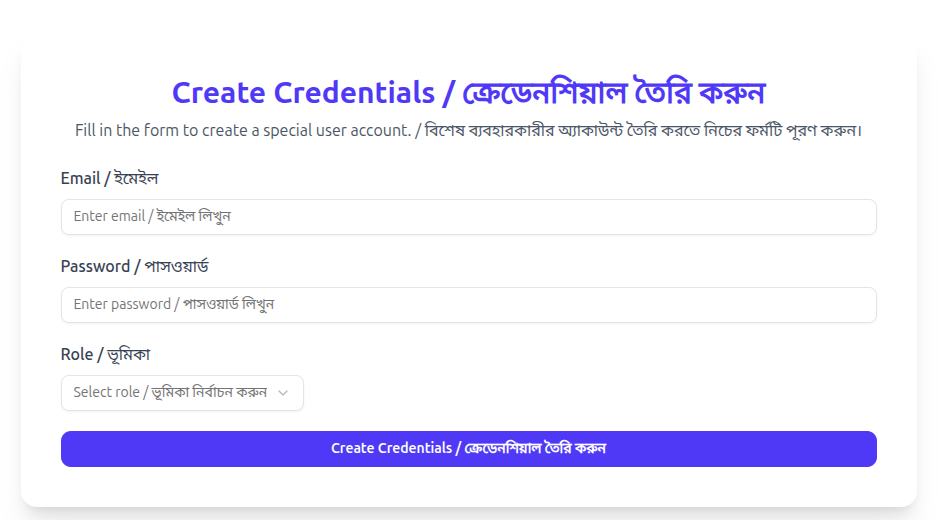
\includegraphics[width=0.75\textwidth]{chapters/chapter4/images/credentail.png}
    \caption{User Credential Creation Interface}
    \label{fig:create_credentials}
\end{figure}

\subsection{System User Monitoring}
A centralized dashboard allows the Admin to monitor all registered officials, their roles, and their account status.

\begin{figure}[H]
    \centering
    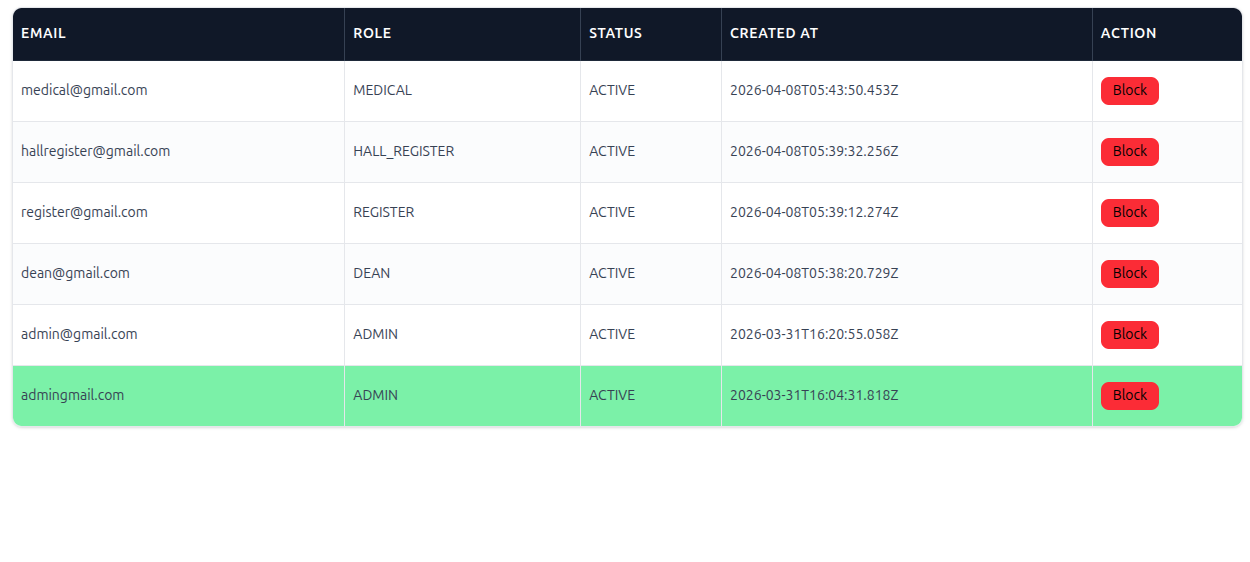
\includegraphics[width=0.9\textwidth]{chapters/chapter4/images/userManagement.png}
    \caption{Administrative User Management Dashboard}
    \label{fig:user_management}
\end{figure}

\begin{itemize}
    \item \textbf{Status Control:} Admins can "Block" or "Unblock" accounts instantly to prevent unauthorized access.
    \item \textbf{Role Identification:} The interface clearly labels the role (e.g., DEAN, REGISTER) and the timestamp of account creation.
\end{itemize}